
\chapter{Knjižnica in gradniki za Orange}

V okviru diplomske naloge smo razvili tri ločene komponente za programerje in
končne uporabnike programa Orange. 

Prva komponenta je programska knjižnica \verb|simple_wbd|, ki
omogoča enostaven dostop do programskega vmesnika indikatorjev in podnebnih
podatkov Svetovne banke. Ta knjižnica je narejena s čim manj odvisnosti in je 
% TODO ali je python z veliko
namenjena splošni uporabi v Python programih. Poudarka pri zasnovi knjižnice 
\verb|simple_wbd| sta predvsem enostavnost razsiritve in zanesljivost. Ta cilja
dosežemo z mehanizmom za vključevanje lastne kode v komponente knjižnice
in mehanizmi za popravljanje ali odstranjevanje pokvarjenih podatkov.

Drugi sestavni del je razširitev knjižnice \verb|simple_wbd| s 
funkcionalnostmi, potrebnimi za lažje delo v programu Orange. To predvsem 
zavzema pretvorbo pridobljenih podatkov v podatkovno tabelo Orange in tabelo 
numpy. Ta sklop je namenjen skriptnemu delu s programom Orange 
\cite{orange_scripting} in je dostopen
kot \verb|api_wrapper| Python modul. 

Tretji sestavni del je grafični vmesnik za uporabo \verb|api_wrapper| modula.
Namen grafičnega vmesnika je omogočiti ne-programerjem dostop do podatkov 
programskega vmesnika Svetovne banke znotraj programa Orange za namen obdelave,
analize in iskanja zakonitosti v podatkih.

\section{Knjižnica simple\_wbd}

Knjižnica \verb|simple_wbd| programerjem olajša dostop do podatkov 
programskega vmesnika Svetovne banke. Glavna lastnost te knjižnice je 
združevanje večjega števila zahtev po podatkih in enostavna predstavitev 
prejetih podatkov. Druga lastnost je pretvorba podatkov iz več dimenzij v 
dvo-dimenzionalno polje, primerno za uporabo v programu Orange. Glavna 
razreda te knjižnice sta \verb|IndicatorAPI| in \verb|ClimateAPI|. Prvi 
omogoča pridobivanje podatkov iz programskega vmesnika indikatorjev, drugi pa 
s programskega vmesnika podnebnih meritev.


Čeprav za dostop do programskega vmesnika Svetovne banke že obstajajo 
rešitve kot sta knjižnici 
\verb|wbdata|\fnurl{https://pypi.python.org/pypi/wbdata} in
\verb|wbpy|\fnurl{https://pypi.python.org/pypi/wbpy/2.0.1}, smo se odločili
za lastno implementacijo podobne knjižnice. Glavni razlog za to je, da
obstoječe rešitve poskušajo čim bolj natančno predstaviti programski
vmesnik Svetovne banke, ne pa olajšati dostop do čim večje količine
podatkov.

Za potrebe te knjižnice smo razvili lastno rešitev za predpomnenje poizvedb,
saj so se bolj splošne rešitve, kot na primer
\verb|vcrpy|\fnurl{https://pypi.python.org/pypi/vcrpy/1.10.0} in
\verb|requests-cache|\fnurl{https://pypi.python.org/pypi/requests-cache}, 
izkazale za prepočasne ko delamo z večjimi količinami podatkov. Naša
rešitev za predpomnenje izkorišča dejstvo da je vsaka poizvedba določena le
z naslovom URL, in da so vsi odgovori oblike JSON. Za vsak URL naredimo novo
datoteko v sistemskem začasnem imeniku, v kateri hranimo serializirane JSON
podatke. Ker se podatki na programskem vmesniku Svetovne banke redko
posodabljajo, smo za čas veljavnosti začasnih datotek izbrali en teden.

% NOTE: serailizacija je baje uredu beseda:
% http://eprints.fri.uni-lj.si/2711/1/63100205-VALENTIN_KRAGELJ-Pregled_in_analiza_tehnologij_za_serializacijo_objektov.pdf

% server query je ful omojen (retarded) mi mamo bolsiga v guiju 

%% % moznost razsiritve z dedovanjem dataset razreda.
%% % 
%% 
%% - omogoča pridobivanje vrednosti za filtre:
%%     - indicator api: drzave in agregati, indikatorji
%%     - climate api: drzave, tipi podatkov, meritveno obdobje 
%% 
%% - Zahteva za podatke vraca dataset objekt ki ponuja surove podatke, ali pa eno
%%   drugo obliko. 2D array ali pa dict.
%% 
%% - Dataset razred lahko tudi poljubno razsirimo.



\subsection{Razred IndicatorAPI}

\verb|IndicatorAPI| je razred namenjen pridobivanju podatkov indikatorjev
razvoja držav. Ker ima programski vmesnik Svetovne banke omejitev koliko 
podatkov lahko prenesemo z eno poizvedbo in nam dovoli tvoriti poizvedbe le za
en indikator na enkrat, smo napisali razred, ki v ozadju tvori in izvede
poizvedbe za vse strani vseh zahtevanih indikatorjev. To poskrbi tako da se po
prvi poizvedbi za en indikator sprehodi čez število preostalih strani 
(Primer \ref{basic_response}), ki so na voljo, in pridobljene podatke večih
strani združi in predstavi kot rezultat ene same poizvedbe. Ta postopek ponovi
za vse zahtevane indikatorje, in njihove rezultate vrne v obliki slovarja, ki 
ima za ključ kodo indikatorja posamezne zahteve.

Poleg tega da skrbi za prenos vseh strani podatkov, tudi beleži število 
izvedenih in število potrebnih poizvedb za celoten prenos. Ta števila se
lahko uporablja za prikaz napredka prenosa podatkov.


Za namene razreda \verb|IndicatorAPI| smo v knjižnici \verb|simple_wbd|
razvili mehanizme za odpravo nekaterih napak omenjenih v poglavju 
\ref{api_gotchas}.

Pri manjkajočih vrednostih držav v poizvedbah za podatke indikatorjev,
poskušamo določiti pravilne vrednosti. To naredimo s pomočjo dveh
slovarjev: prvi slika kode držav v imena, drugi pa imena držav v kode. V
primeru manjkajoče vrednosti kode ali imena, poskušamo to prebrati iz enega
od naštetih slovarjev. Če nam ne uspe ugotoviti manjkajočih vrednosti,
trenutni vnos odstranimo iz rezultata poizvedbe.

Drugi tip napak, ki ga lahko delno popravimo, so napačne vrednosti v polju
\verb|date| v poizvedbah za podatke indikatorjev. Ker lahko v temu polju
pričakujemo poljubno besedilo, dela naš pretvornik za polje \verb|date| v 
datum, tako da poskuša v datum pretvoriti čim daljšo predpono besedila.
Če nam ne uspe besedila pretvoriti v veljaven datum, trenutni vnos odstranimo
iz rezultata poizvedbe.


\ \\
Glavne metode ki jih ponuja razred IndicatorAPI so:

\begin{description}  
\item [get\_indicators] za pridobivanje seznama indikatorjev s kodami, imeni
      in opisi,
\item [get\_countries] za pridobivanje seznama držav z metapodatki,
\item [get\_dataset] za pridobivanje podatkov za indikatorjev.
\end{description}


\subsubsection{Razred IndicatorDataset}

Razred \verb|IndikatorDataset| je osnovni razred v katerem dobimo zahtevane podatke
indikatorjev. Ta razred vsebuje vse potrebne metode in podatke za predstavitev
rezultatov programskega vmesnika, na dva glavna načina; kot slovar slovarjev in
dvo dimenzionalen seznam. Poleg omenjenih načinov predstavitve podatkov lahko
dostopamo tudi do neobdelanih podatkov prejetih iz programskega vmesnika za
vsako poizvedbo posebej.


Posamezne vrednosti teh podatkov so določene z državo, časovno komponento, in
kodo indikatorja. Te podatke lahko predstavimo na dva glavna načina:

 - kot gnezdeni slovar, kjer je na prvem nivoju ime indikatorja, na drugem
   drzava, in na tretjem nivoju casovna komponenta.

 - Kot dvo-dimenzionalno polje, kjer imamo v vrsticah eno oznako, v stolpcih
   pa kartezicni produkt ostalih dveh. ponujene moznosti so:
   - vrstice = drzava, stolpci = cas x indikator
   - vrstice = cas, stolpci = drzava x indikator


Indicator



% notes:
% 3 dimenzije: cas, drzava, indikator > vrednost
% 
% lahko damo v:
% 
% 
%    \    drzava x indikator
%   cas
% 
%  ali: 
% 
%    \    cas x indikator
% drzava
% 


\subsubsection{Primeri uporabe}





\subsection{Pomcnik ClimateAPI}

IndicatorAPI je 


api dovoli le podatke za en tip za eno vrsto obdobja in eno drzavo hkrati.
mi naredim kartezicni produkt med vsemi temi zgradimo vse url-je in naredimo
vse potrebne poizvedbe za pridobitev podatkov.



\subsubsection{Razred IndicatorDataset}

Isto kot pri indicator apiju
ko zelimo dobiti polje v obliki casovne vrste:
 - pridobivanje datuma iz polja 'date'
   - ob neveljavnih stringih probamo upostevati le zacetni del.
     - za text za  obdobje  '2002 - 2006' bomo uporabili le datum 2002 
   - neveljavne stringe kot so ``most recent value'' ignoriramo.




as\_dict 

glede na poizvedbo dobimo tu gnezden slovar s polji

drzava / tip podatkov / tip casovnega obdobja / vrednost casovnega obdobja / vrednost

as\_list

% notes:
% 3 dimenzije: cas (decade,year,month), drzava, tip (pr/ tas)
% 
% lahko damo v poljubno konfiguracijo z nastetimi elementi v stolpcu
% 
% stolpci = [drzava, cas] => vrstice = tip ... naredi kartezicni produkt



\section{api\_wrapper}

% doda as orange table in as numpy obema indikator apiju in climate apiju.


razširitev simple wbd vmesnikov z dedovanjem pravega dataset razreda.

\begin{verbatim}

class ClimateDataset(simple_wbd.ClimateDataset):
    
    def as_numpy(self):
        raise NotImplemented()
    
    def as_orange_table(self):
        raise NotImplemented()

class ClimateAPI(simple_wbd.ClimateAPI):

    def __init__(self):
        super().__init__(ClimateDataset)
\end{verbatim}


- razsiri as\_list v as\_numpy\_array ki tudi odstrani vse stolpce ki nimajo 
  veljavne vrednosti.

- doda as orange table ki numpy array spremeni v orange tabelo.
  - za indikator api doda se metapodatke drzav ko ne prikazujemo v obliki casovne vrste.


api vrapper je tudi zelo uporaben za skriptno uporaba programa Orange 
(referenca http://www.jmlr.org/papers/volume14/demsar13a/demsar13a.pdf)

in tukaj si lahko vsak programer sam oblikuje podatke v katerokoli zeljeno obliko.






\section{Graficni vmesnik}


 
nova skupina data sets 
 - v katero je mogoce dodati nove gradnike za druge programske vmesnike.

2 gradnika - wb indicators in wb climate

- lazja uporaba apija
- vecja preglednost


za oba gradniko smo razvili in uporabili base class - skupni podatki

- razvili smo tudi gradnik za gnezned prikaz urejenih slovarjev.
  ta se uporablja za prikaz drzav po kontinentih v climate gradniku,
  in za prikaz drzav in skupin drzav in drugih agregatov v gradniku
  indicators.


za te gradnike smo tudi napisali enotske teste.


\begin{figure}
  \begin{center}
    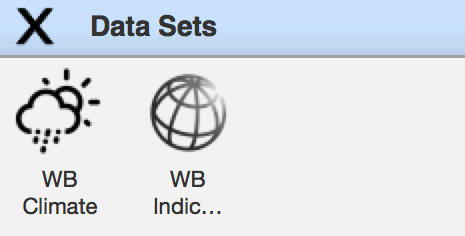
\includegraphics[width=4cm]{pic/data_sets_group.png}
  \end{center}
  \caption{Skupina gradnikov data sets}
  \label{drevo}
\end{figure} 


\subsection{wb indicators gradnik}

za sestavo smo si pomagali z gradniki Orange.gui 

elementi gradnika

2 osnovna filtra: 

- izbor indikatorjev ki se pokazejo v seznamu all/common/featured 
  ki ustreza seznamu indikatorjev na strani: 
  all - vse (tudi nekateri ki jih na strani ni nastetih)
  common - http://data.worldbank.org/indicator?tab=all
  featured - http://data.worldbank.org/indicator?tab=featured
- text filter

gradnik ima sistem za prikaz (progress bar?) 

moznost izbire tipa izhoda (countries in time series - opis)

\begin{figure}
\begin{center}
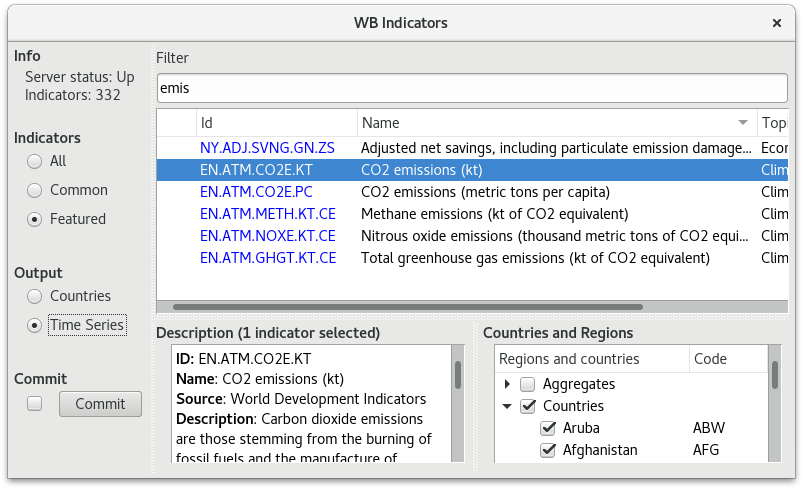
\includegraphics[width=12cm]{pic/co2_temp_indicator_selection.png}
\end{center}
\caption{Odločitveno drevo za izbor primerne metode.}
\label{co2_temp_indicator}
\end{figure} 



\subsection{wb climate gradnik}

dovoli izbiro posameznih drzav 

moznost izbire tipa izhoda (countries in time series - opis)
za razliko od indikator apija tukaj nismo dodali metapodatkov drzav 



\begin{figure}
\begin{center}
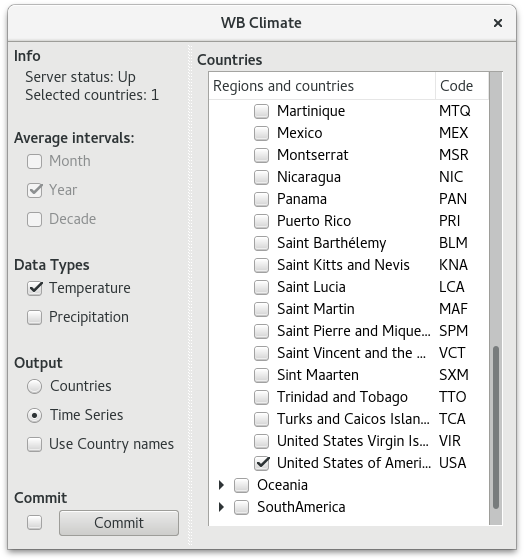
\includegraphics[width=12cm]{pic/co2_temp_climate_selection.png}
\end{center}
\caption{Odločitveno drevo za izbor primerne metode.}
\label{co2_temp_indicator}
\end{figure} 
